\documentclass{beamer}
\usetheme[deutsch]{KIT}

\usepackage[utf8]{inputenc}
\usepackage[T1]{fontenc}
\usepackage{listings}
\usepackage{pgfplots}
\usepackage{babel}
\usepackage{tikz,calc,ifthen}
\usepackage{mathtools}
\usepackage[normalem]{ulem}
\usepackage{graphicx}
\usepackage{subfig}
\usepackage{booktabs}
\usepackage{pgfplotstable}

% Colors
\definecolor{firmBlue}     {rgb}{0.6,  0.6, 1   }
\definecolor{firmCyan}     {rgb}{0.8,  1,   1   }
\definecolor{firmDarkBlue} {rgb}{0.4,  0.4, 1   }
\definecolor{firmGreen}    {rgb}{0.42, 1,   0.42}
\definecolor{firmDarkGreen}{rgb}{0,    0.5, 0   }
\definecolor{firmRed}      {rgb}{1,    0.6, 0.6 }
\definecolor{firmViolet}   {rgb}{0.5,  0,   0.5}
\definecolor{firmYellow}   {rgb}{1,    1,   0.6 }

% Nodes
\tikzstyle{graph}      = [fill=lightgray]
\tikzstyle{firm}       = [draw, fill=white]
\tikzstyle{block}      = [draw, fill=yellow]
\tikzstyle{const}      = [draw, fill=firmCyan]
\tikzstyle{control}    = [draw, fill=firmRed]
\tikzstyle{memory}     = [draw, fill=firmBlue]
\tikzstyle{phi}        = [draw, fill=green]
\tikzstyle{proj}       = [draw, fill=firmYellow]
\tikzstyle{start}      = [draw, fill=firmDarkBlue]

% Edges
\tikzstyle{dataDependency}    = [thick, -latex]
\tikzstyle{controlDependency} = [dataDependency, color=red]
\tikzstyle{memoryDependency}  = [dataDependency, color=firmDarkBlue]
\tikzstyle{keep}              = [dataDependency, color=firmViolet]
\tikzstyle{dependency}        = [dataDependency, color=firmDarkGreen]


\usetikzlibrary{positioning,calc,arrows,shapes}
\tikzset{
  every node/.style={transform shape},
  auto,
  block/.style={align=center,rectangle,draw,minimum height=20pt,minimum width=30pt},
  >=triangle 60,
  alt/.code args={<#1>#2#3}{%
      \alt<#1>{\pgfkeysalso{#2}}{\pgfkeysalso{#3}}
  },
  beameralert/.style={alt=<#1>{color=green!80!black}{}},
  mythick/.style={line width=1.4pt}
}

\newcommand*{\maxwidthofm}[2]{\maxof{\widthof{$#1$}}{\widthof{$#2$}}}
\newcommand<>*{\robustaltm}[2]{
  \alt#3
  {\mathmakebox[\maxwidthofm{#1}{#2}]{#1}\vphantom{#1#2}}
    {\mathmakebox[\maxwidthofm{#1}{#2}]{#2}\vphantom{#1#2}}
}

\newcommand<>*{\nodealert}[1]{\only#2{\draw[overlay,mythick,color=green!80!black] (#1.north west) rectangle (#1.south east)}}

\title{Improved integer conversion optimisation and VHDL code generation based on bit-width analysis}
\author{Marcel Hollerbach}
\subtitle{\insertauthor}
\institute[IPD]{Lehrstuhl Programmierparadigmen, IPD Snelting}
\date{29.10.2018}
\KITtitleimage{cover.png}

\begin{document}

\begin{frame}
  \maketitle
\end{frame}


\begin{frame}[fragile]{Das Ziel}
\begin{lstlisting}
int arr[4];

for (int i = 0; i < 4; i++) {

	int x = i*i;      
	int y = (i << 4); 
	int res = x + y;  
	arr[i] = res;
}
\end{lstlisting}
Wie viele bits nutzen \textit{i}, \textit{x}, \textit{y}, \textit{res}? \newline
\end{frame}

\begin{frame}{Was ist eine Bitbreite}
\begin{center}
	\begin{definition}{bitbreite}
		(stable\_bits, is\_positive)
	\end{definition}
\end{center}

\begin{tabular}{ c c | c c c c c c c c | c c }
	mode & value & \multicolumn{8}{c|}{bit representation} & stable\_bits & is\_positive \\
	\hline
	\hline
	Bs & 5     & \color{red}0 & \color {red}0 & \color{red}0 & \color{red}0 & 0 & 1 & 0 & 1 & 4 & true\\
	Bs & -2    & \color{red}1 & \color{red}1 & \color{red}1 & \color{red}1 & \color{red}1 & \color{red}1 & 1 & 0 & 6 & false\\
    Bu & 5     & \color{red}0 & \color{red}0 & \color{red}0 & \color{red}0 & \color{red}0 & 1 & 0 & 1 & 5 & - \\
\end{tabular}

\end{frame}

%\begin{frame}[fragile]{Das Ziel}
%\begin{lstlisting}
%\begin{tabular}{ c c }
%Variable & Verbrauch \\
%i & 3 \\
%x & 6 \\
%y & 7 \\
%res & 8 \\
%\end{tabular}
%\end{lstlisting}
%\end{frame}

\begin{frame}{libFIRM}
\begin{columns}
	\begin{column}{0.5\textwidth}
		\begin{enumerate}
			\item Integer-modes sind genutzt
			\item Nutzung von Arithmetische/Logische ausdruecke
			\item Behandlung von Confirm knoten
		\end{enumerate}
	\end{column}
		\begin{column}{0.5\textwidth}  %%<--- here
			\begin{center}
				\begin{tikzpicture}
				\node[graph]{
					\begin{tikzpicture}[remember picture]
					\node[block] (startblock) {
						\begin{tikzpicture}
						\node[firm]    (const0) at (0,2) {Const : 0};
						\node[phi]     (phi)    at (-1,1) {Phi};
						\node[firm]    (const1) at (1,1) {Const : 1};
						\node[firm]    (add)    at (0,0) {Add};
						\node[firm]    (cmp)        at ( 0,-1) {Cmp less\_equal};
						\node[control] (cond)       at ( 0,-2) {Cond};
						\node[control] (false)      at (-1,-3) {False};
						\node[control] (true)       at ( 1,-3) {True};
						
						\draw[dataDependency]    (add.60)      -- ++(0,0.1) -| (const1);
						\draw[dataDependency]    (add.120)     -- ++(0,0.1) -| (phi);
						\draw[dataDependency]    (phi.60)      -- ++(0,0.1) -| (const0);
						\draw[dataDependency]    (phi.120)     -- ++(0,0.1) -- ++(-1,0) -- ++(0,-2) -| (add.240);
						\draw[dataDependency]    (cmp.62)     --              (add.300);
						\draw[dataDependency]    (cond)        --              (cmp);
						\draw[controlDependency] (false.north) -- ++(0,0.1) -| (cond.240);
						\draw[controlDependency] (true.north)  -- ++(0,0.1) -| (cond.300);
						
						\end{tikzpicture}
					};
				\end{tikzpicture}
			};
		\end{tikzpicture}
		\end{center}
	\end{column}
\end{columns}
\end{frame}

\begin{frame}{libFIRM}
\begin{columns}
	\begin{column}{0.5\textwidth}
		Confirm-node
		\newline
		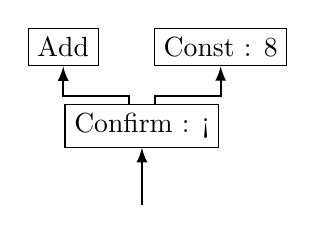
\begin{tikzpicture}
			\node[firm]    (add)    at (-1,1) {Add};
			\node[firm]    (const0) at (1,1) {Const : 8};
			\node[firm]    (confirm) at (0,0) {Confirm : <};
			\draw[dataDependency]    (confirm.60)      -- ++(0,0.1) -| (const0);
			\draw[dataDependency]    (confirm.120)     -- ++(0,0.1) -| (add);
			\draw[dataDependency]    (0,-1) -- (confirm);
		\end{tikzpicture}
		%FIXME
	\end{column}
	\begin{column}{0.5\textwidth}  %%<--- here
		Convertion-node
		\newline
		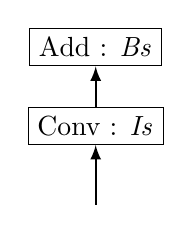
\begin{tikzpicture}
		\node[firm]    (add)    at (0,1) {Add : \textit{Bs}};
		\node[firm]    (conv) at (0,0) {Conv : \textit{Is}};
		\draw[dataDependency]    (conv) -- (add);
		\draw[dataDependency]    (0,-1) -- (conv);
		\end{tikzpicture}
		%FIXME
	\end{column}
\end{columns}
\end{frame}



\begin{frame}{Analyse}
Implementiert mit worklist appraoch.
\begin{center}
	\begin{tabular}{ l | c }
		op & stable bits \\
		\hline
		add & $max(min(a_{stable}, b_{stable}) - 1, 0)$ \\
		minus &  $max(a_{stable} - 1, 0) $ \\
		sub &  $max(min(a_{stable}, b_{stable}) - 1, 0) $ \\
		mul &  $max(2*mode - ( b_{stable} + a_{stable} ), 0)  $ \\
		div &  
		$ 
		\left\{
		\begin{array}{l}
		a_{stable}\\ 
		max(a_{stable} - 1, 0)
		\end{array}
		\begin{array}{l}
		, \neg mode\text{ is signed} \\ 
		, \text{otherwise}.
		\end{array}
		\right.$\\
		mod & 
		$
		\lfloor log2(max(a))\rfloor
		$
		\\
	\end{tabular}
\end{center}
\end{frame}

\begin{frame}{Analyse 2}
\begin{center}
	$add(const(5), x) \equiv max(min(4, 5) - 1, 0) \equiv 3$
\newline
\newline
\newline
\begin{tabular}{ c | c c }
	stable\_bits & min & max \\
	\hline
	\hline
	5 & -4 & +3 \\
	4 & -8 & +7\\
	3 & -16 & +15 \\
\end{tabular}
\end{center}
\end{frame}

\begin{frame}{Schleifen im Graphen}
Mit möglichem Confirm-node:
\begin{center}
\begin{tikzpicture}
\node[graph]{
	\begin{tikzpicture}[remember picture]
	\node[block] (startblock) {
		\begin{tikzpicture}
		\node[firm]    (const0) at (1,2) {Const : 0};
		\node[phi]     (phi)    at (-1,1) {Phi};
		\node[firm]    (cmp)        at ( 0,-1) {Cmp less\_equal};
		\node[control] (cond)       at ( 0,-2) {Cond};
		\node[control] (false)      at ( 1,-3) {False};
		\node[control] (true)       at (-1,-3) {True};
		
		\draw[dataDependency]    (phi.60)      -- ++(0,0.1) -| (const0);
		\draw[dataDependency]    (cmp.60)        -- ++(0,0.1) -| (phi.300);
		\draw[dataDependency]    (cond)        --              (cmp);
		\draw[controlDependency] (false.north) -- ++(0,0.1) -| (cond.300);
		\draw[controlDependency] (true.north)  -- ++(0,0.1) -| (cond.240);
		\end{tikzpicture}
	};
	\node[block, anchor=east] (end) at ($(startblock.west) + (-1,0)$) {
		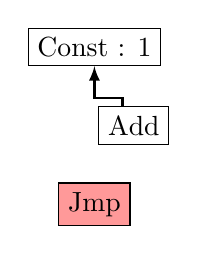
\begin{tikzpicture}
		\node[firm]    (const1) at (0,0) {Const : 1};
		\node[firm]    (add) at (0.5,-1) {Add};
		\node[control] (ret) at (0,-2) {Jmp};
		
		
		\draw[dataDependency] (add.120) -- ++(0,0.1) -| (const1);
		\end{tikzpicture}
	};
	\begin{scope}									
		\draw[dataDependency] (add.60) -- ++(0,0.1) -| (phi);
		\draw[dataDependency]  (phi)-- ++(0,+0.49) -- ++(-4.5,0) -- ++(0,-2.5) -| (add.240);
	\end{scope}
	
	
\end{tikzpicture}
};	
\end{tikzpicture}
\end{center}
\end{frame}


\begin{frame}{Schleifen im Graphen}
Ohne möglichen Confirm-node:
\begin{center}
\begin{tikzpicture}
	\node[graph]{
		\begin{tikzpicture}[remember picture]
			\node[block] (startblock) {
				\begin{tikzpicture}
				\node[firm]    (const0) at (1,2) {Const : 0};
				\node[phi]     (phi)    at (-1,1) {Phi};
				\node[firm]    (conv)    at (0,0) {Conv};
				\node[firm]    (cmp)        at ( 0,-1) {Cmp less\_equal};
				\node[control] (cond)       at ( 0,-2) {Cond};
				\node[control] (false)      at ( 1,-3) {False};
				\node[control] (true)       at (-1,-3) {True};
				
				\draw[dataDependency]    (phi.60)      -- ++(0,0.1) -| (const0);
				\draw[dataDependency]    (conv.60)        -- ++(0,0.1) -| (phi.300);
				\draw[dataDependency]    (cmp)     --              (conv);
				\draw[dataDependency]    (cond)        --              (cmp);
				\draw[controlDependency] (false.north) -- ++(0,0.1) -| (cond.300);
				\draw[controlDependency] (true.north)  -- ++(0,0.1) -| (cond.240);
				\end{tikzpicture}
			};
			\node[block, anchor=east] (end) at ($(startblock.west) + (-1,0)$) {
				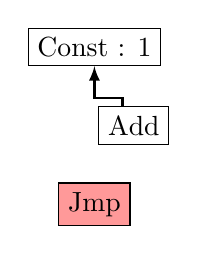
\begin{tikzpicture}
				\node[firm]    (const1) at (0,0) {Const : 1};
				\node[firm]    (add) at (0.5,-1) {Add};
				\node[control] (ret) at (0,-2) {Jmp};
				

				\draw[dataDependency] (add.120) -- ++(0,0.1) -| (const1);
				\end{tikzpicture}
			};
			\begin{scope}									
				\draw[dataDependency] (add.60) -- ++(0,0.1) -| (phi);
				\draw[dataDependency]  (phi)-- ++(0,+0.49) -- ++(-4.5,0) -- ++(0,-2.5) -| (add.240);
			\end{scope}


		\end{tikzpicture}
	};	
\end{tikzpicture}
\end{center}
\end{frame}

\begin{frame}{Zusätzliche Confirm-nodes}
\begin{columns}
	\begin{column}{0.5\textwidth}
		Stable bits von add:
		\begin{enumerate}
			\item (32, true)
			\item (30, true)
			\item (29, true)
			\item (28, true) [7,-8]
			\item \color{red}(27, true) [15,-16] -> \color{darkgray}insert Confirms
		\end{enumerate}
	\end{column}
	\begin{column}{0.5\textwidth}  %%<--- here
	\begin{tikzpicture}
		\node[graph]{
			\begin{tikzpicture}[remember picture]
				\node[block] (startblock) {
					\begin{tikzpicture}
						\node[firm]    (const0) at (0.5,2) {Const : 0};
						\node[phi]     (phi)    at (-0.4,1) {Phi};
						\node[firm]    (conv)    at (0,0) {Conv};
						\node[firm]    (const2)      at (2,0) {Const : 10};
						\node[firm]    (cmp)        at ( 0,-1) {Cmp less\_equal};
						\node[control] (cond)       at ( 0,-2) {Cond};
						\node[control] (false)      at ( 1,-3) {False};
						\node[control] (true)       at (-1,-3) {True};
						
						\draw[dataDependency]    (phi.60)      --  ++(0,0.1) -| (const0);
						\draw[dataDependency]    (conv.120)        --  ++(0,0.1) -| (phi.300);
						\draw[dataDependency]    (-2.0,0.34)        --  ++(0,0.0) -| (phi.240);
						\draw[thick]             (-2.0,1.45)        --  ++(0,0.0) -| (phi.120);
						\draw[dataDependency]    (cmp)     --              (conv);
						\draw[dataDependency]    (cmp.60)     --    ++(0,0.1)-| (const2);
						\draw[dataDependency]    (cond)        --              (cmp);
						\draw[controlDependency] (false.north) -- ++(0,0.1) -| (cond.300);
						\draw[controlDependency] (true.north)  -- ++(0,0.1) -| (cond.240);
					\end{tikzpicture}
				};
			\end{tikzpicture}
		};	
	\end{tikzpicture}
	\end{column}
\end{columns}
\end{frame}


\begin{frame}{Zusätzliche Confirm-nodes}
\begin{columns}
	\begin{column}{0.5\textwidth}
		Stable bits von add:
		\begin{enumerate}
			\item (32, true)
			\item (30, true)
			\item (29, true)
			\item (28, true) [7,-8]
			\item \color{red}(27, true) [15,-16] -> \color{darkgray}insert Confirms
		\end{enumerate}
	\end{column}
	\begin{column}{0.5\textwidth}  %%<--- here
	\begin{tikzpicture}
		\node[graph]{
			\begin{tikzpicture}[remember picture]
			\node[block] (startblock) {
				\begin{tikzpicture}
				\node[firm]    (const0) at (0.5,2) {Const : 0};
				\node[phi]     (phi)    at (-0.4,1) {Phi};
				\node[firm]    (confirm)    at (0,0) {confirm};
				\node[firm]    (conv)    at (0,-1) {Conv};
				\node[firm]    (const2)      at (2,-1) {Const : 10};
				\node[firm]    (cmp)        at ( 0,-2) {Cmp less\_equal};
				\node[control] (cond)       at ( 0,-3) {Cond};
				\node[control] (false)      at ( 1,-4) {False};
				\node[control] (true)       at (-1,-4) {True};
				
				\draw[dataDependency]    (phi.60)      --  ++(0,0.1) -| (const0);
				\draw[dataDependency]    (conv) -- (confirm);
				\draw[dataDependency]    (confirm.120)        --  ++(0,0.1) -| (phi.300);
				\draw[dataDependency]    (-2.0,-0.55)        --  ++(0,0.0) -| (confirm.240);
				\draw[thick]             (-2.0,1.45)        --  ++(0,0.0) -| (phi.120);
				\draw[dataDependency]    (cmp)     --              (conv);
				\draw[dataDependency]    (cmp.60)     --    ++(0,0.1)-| (const2);
				\draw[dataDependency]    (cond)        --              (cmp);
				\draw[controlDependency] (false.north) -- ++(0,0.1) -| (cond.300);
				\draw[controlDependency] (true.north)  -- ++(0,0.1) -| (cond.240);
				\end{tikzpicture}
			};
		\end{tikzpicture}
		};	
		\end{tikzpicture}
	\end{column}
\end{columns}
\end{frame}

\begin{frame}[fragile]{Zusätzliche Confirm-nodes (Beispiel)}
\begin{lstlisting}
unsinged int l = 20;

for (int i = 0; i < l; i++) {
  data[i] = calculate(i);
}
\end{lstlisting}
\end{frame}


\begin{frame}{Verwendungen der Analyse}
\begin{enumerate}
	\item Conversion-node Entfernung (Cmp)
	\item VHDL Generierung
\end{enumerate}
\end{frame}


\begin{frame}{Conversion-node Entfernung (Cmp)}

\begin{columns}
	\begin{column}{0.5\textwidth}
		\textbf{Idee:}
		\begin{enumerate}
			\item Entfernen von Conv-node
			\item Unterstützung anderer Analysen
		\end{enumerate}
		\textbf{Voraussetzung:}
		\begin{enumerate}
			\item Cmp-node mit Const-node und Conv-node
			\item Used bits von Conv-node muss unverändert sein
		\end{enumerate}
	\end{column}
	\begin{column}{0.5\textwidth}  %%<--- here
		\begin{center}
\begin{tikzpicture}[scale=.7]
\node[graph]{
\begin{tikzpicture}[remember picture]
\node[block] (startblock) {
\begin{tikzpicture}


\node[firm]    (conv) at (-1,2) {Conv};
\node[firm]    (const) at (1,2) {Const};
\node[firm]    (cmp)    at (0,1) {Cmp};
\node[firm]    (cond)    at (0,0) {Cond};

\draw[dataDependency]    (conv.north)   -- ++(0,0) -| (-1,3);	

\draw[dataDependency]    (cmp.60)      -- ++(0,0.1) -| (const);
\draw[dataDependency]    (cmp.120)      -- ++(0,0.1) -| (conv);
\draw[dataDependency]    (cond.north)     -- ++(0,0.1) -| (cmp.south);

\end{tikzpicture}
};
\end{tikzpicture}
};
\end{tikzpicture}
		\end{center}
	\end{column}
\end{columns}
\end{frame}

\begin{frame}{Conversion-node Entfernung (Cmp)}

\begin{columns}
	\begin{column}{0.5\textwidth}
		\textbf{Optimierung:}
		\begin{enumerate}
			\item Conv-node entfernen
			\item Mode von Const anpassen
		\end{enumerate}
	\end{column}
	\begin{column}{0.5\textwidth}  %%<--- here
		\begin{center}
\begin{tikzpicture}[scale=.7]
\node[graph]{
	\begin{tikzpicture}[remember picture]
	\node[block] (startblock) {
		\begin{tikzpicture}
		
		
		\node[firm]    (const) at (1,2) {Const};
		\node[firm]    (cmp)    at (0,1) {Cmp};
		\node[firm]    (cond)    at (0,0) {Cond};
		
		\draw[dataDependency]    (cmp.60)      -- ++(0,0.1) -| (const);
		\draw[dataDependency]    (cmp.120)      -- ++(0,0.1) -| (-1,1.9);
		\draw[dataDependency]    (cond.north)     -- ++(0,0.1) -| (cmp.south);
		
		\end{tikzpicture}
	};
\end{tikzpicture}
};
\end{tikzpicture}
		\end{center}
	\end{column}
\end{columns}
\end{frame}
\begin{frame}[fragile]{Evaluierung der Optimierung}
Verbesserte Bitbreite:
\begin{figure}
	\centering
	\pgfplotstabletypeset[col sep=comma, fixed, zerofill, precision=4,
	columns={Library, mode usage(1), bitwidth usage(1)},
	columns/Library/.style={column type=l,string type},
	every head row/.style={after row=\midrule},
	every last row/.style={after row=\bottomrule}
	]{../thesis/data.csv}
\end{figure}
Erfahrungen:
\begin{enumerate}
	\item Loop-Unroller verbessert sich
	\item Geringe Auswirkung auf die Assembler Generierung
\end{enumerate}
\end{frame}
%\begin{frame}{Conversion-node entfernung (arithmetical)}
	\begin{columns}
		\begin{column}{0.5\textwidth}
			\textbf{Idee:}
			\begin{enumerate}
				\item Verschieben der Conv knoten
				\item Späteres entfernen durch Conversion-node entfernung
			\end{enumerate}
			\textbf{Voraussetzung:}
			\begin{enumerate}
				\item Arithmetical node mit Const-node und Conv-node
				\item Bitbreite von Conv-node muss unverändert sein
			\end{enumerate}
		\end{column}
		\begin{column}{0.5\textwidth}  %%<--- here
			\begin{figure}
	\centering
	\begin{tikzpicture}[scale=.7]
		\node[graph]{
			\begin{tikzpicture}[remember picture]
				\node[block] (startblock) {
					\begin{tikzpicture}		
						\node[firm]    (const) at (-1,1) {Const};
						\node[firm]    (conv) at (1,1) {Conv};
						\node[firm]    (add)    at (0,0) {Add};
						
						\draw[dataDependency]    (conv.north)    -- ++(0,0) -| (1,2);	
						\draw[dataDependency]    (add.120)  -- ++(0,0.1) -| (const);
						\draw[dataDependency]    (add.60) -- ++(0,0.1) -| (conv);
					\end{tikzpicture}
				};
			\end{tikzpicture}
		};
	\end{tikzpicture}
\caption{A subgraph where the arithmetical optimization can be performed.}
\label{fig:example:arithmetical_opt}
\end{figure}
		\end{column}
	\end{columns}
\end{frame}

\begin{frame}{Conversion-node entfernung (arithmetical)}

	\begin{columns}
		\begin{column}{0.5\textwidth}
			\textbf{Optimierung:}
			\begin{enumerate}
				\item Conv-node nach arithmetical-node
				\item mode von arithmetical-node \& Const-node anpassen
			\end{enumerate}
		\end{column}
		\begin{column}{0.5\textwidth}  %%<--- here
			FIXME
		\end{column}
	\end{columns}
\end{frame}
\begin{frame}{Conversion-node entfernung (arithmetical)}
Probleme:
\begin{enumerate}
	\item Kommt in der Praxis nicht vor
\end{enumerate}
\end{frame}



\begin{frame}[fragile]{VHDL Generierung}
Vorgehen:
\begin{enumerate}
	\item C Quellcode kompilieren zu IR Format
	\item Kompiliere IR Format zu VHDL
\end{enumerate}

Beispielcode:
\begin{lstlisting}
variable node199 : signed(31 downto 0):= (others => '0'); 
variable node194 : signed(31 downto 0):= (others => '0'); 
variable node193 : unsigned(31 downto 0):= (others => '0'); 
[...]
node199 := node172 xor node198;
node194 := node199 + node193;
node193 := unsigned (resize(node194,32));
\end{lstlisting}
\end{frame}

\begin{frame}[fragile]{VHDL Generierung}
Idee:
\begin{enumerate}
	\item Nutzung der minimalen Variablenbreite
	\item Dadurch verminderte LUT Anzahl
\end{enumerate}

Beispielcode:
\begin{lstlisting}
variable node199 : signed(9 downto 0):= (others => '0'); 
variable node194 : signed(16 downto 0):= (others => '0'); 
variable node193 : unsigned(31 downto 0):= (others => '0'); 
[...]
node199 := resize(node172,10) xor resize(node19,10);	
node194 := resize(node199,17) + resize(node193,17);	
node193 := resize(unsigned(resize(node194,32)),32);	
\end{lstlisting}
\end{frame}

\begin{frame}{VHDL Generierung (Evaluation)}

\textbf{Vorgehen der Evaluation:}
\begin{enumerate}
	\item Übersetzen von C Quellcode zu VHDL ohne Optimierung
	\item Nochmaliges Übersetzen mit Optimierung
	\item Vergleich der beiden Ergebnisse
\end{enumerate}
\end{frame}

\begin{frame}{VHDL Generierung (Evaluation)}
\begin{tabular}{c | c | c | c}
	IDE    & Unoptimiert & Optimiert & Hand optimiert \\
	\hline
	Vivado & 108 & 112 & 109 \\
	Quartus & 54 & 54 & - \\
\end{tabular}
\newline
\newline
\newline
\newline
\newline
\textbf{Testcode:} 
\newline
\begin{tabular}{ c | c | c }
	& Unoptimiert & Optimiert \\
	\hline
	Genutzte Bitbreite & 928 & 609 \\
\end{tabular}
\end{frame}

\chapter{Conclusion}\label{sec:conclusion}

\section{Assembler generation}
The previous chapter showed that the optimizations are not that helpful on decoder code. This thesis was done for evaluating decoder code, so no others projects have been checked. However, other projects like direct UI or CLI implementations also could be evaluated, since the patterns from decoding code are quite different to ui codes. Without evaluating others, we can say, that the optimization for dropping conversion nodes from the graph is not that helpful.

\section{vhdl generation}
Its similar to the assembler generation. There is no obvious improvement over the not optimized VHDL code. However, its very hard to see real differences due to the inability to understand the real differences in the bitstream. A open bitstream standard would help here, since the projects then could be compared on the lowest possible hardware layer.
\section{Further improvements}
\subsection{Widening \& Narrowing}

Widening and Narrowing is a technique that tries to achieve the same or slightly worse results, by maintaining a better runtime. Here are a few things that could be done in this analysis to achive this. However, the time was short and thus the following is only thought about, but not yet implemented.

\paragraph{Widening not terminating loops}
There is the theoretical question of when we are able to predict that a loop will terminate before the whole bitwidth is used or not. The question for this analysis is quite simple, if there is a Compare node in the loop, and it is defining a upper bound, then we might find a upper bound when we insert the confirm node there as described in \ref{upper_bound_insert_confirm}. If there is no Confirm node, and no Compare node, then there is no chance for the loop to terminate. And thus we might want to wide our stable bits to 0.

\paragraph{Narrowing for arithmetical chains}
As explained in \ref{VRP_king}, the VRP returns a more accurate result for arithmetical chains. A arithmetical chain can be defined as a set of arithmetical nodes, where each node has a successor which is a arithmetical node.

The problem with arithmetical operations is within the bitwidth analysis is, is that we need to calculate the worst case in terms of bit usage. As an example, two operands with the ranges $[0..2]$ and $[0..4]$ will result in the range $[0..6]$. However, we are in a bitwidth analysis here, which means the ranges here are always rounded up to the next power of two. This means for our example, that the two operands will have the same ranges, but the result of the addition will be $[0..8]$. In higher bit ranges, the lose is even bigger.

The problem can be fixed, by calculating the result for a arithmetical node as the bitwidth information, as well as the exact range. The successor of the node can then use the exact range instead of the bitwidth info for calculating its results. Thus we end up in the same result as the VRP.

\section{Additional analyzer usage}
\paragraph{More conversion nodes}
In this thesis we looked at removing the conversion nodes where we can. However, in some situations it might makes sense to insert more conversion nodes where most of a mode is not used, and thus the reduction to a smaller mode would be possible. This might enables the compiler to better use the available registers. As an example, a simple for loop might only iterate in the ranges of a 8 bit number. And thus the 8 bit registers of the hardware could be used instead of the bigger 32 bit registers. A additional situation where this might makes sense is a shift operation on 32bit systems , as a long shift is very complex on a 32 bit architecture, and might not be required.

\end{document}
